\begin{figure}[htbp]
\centering
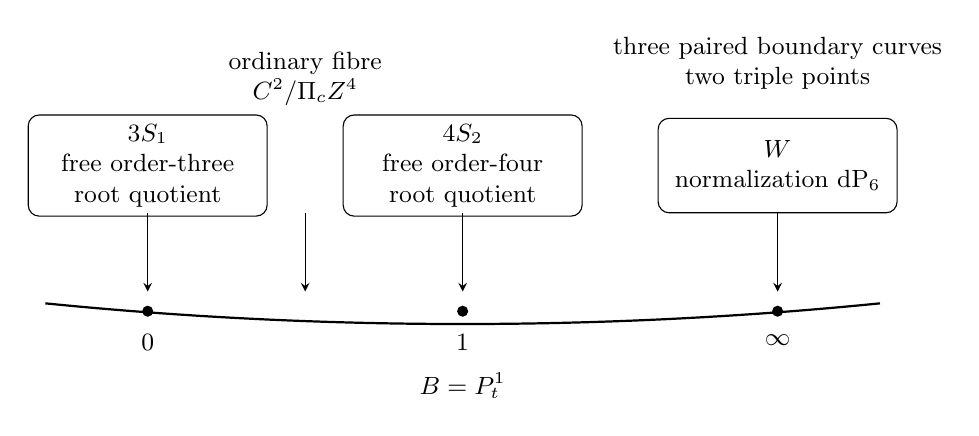
\begin{tikzpicture}[x=1cm,y=1cm,>=stealth,font=\small]
\draw[thick] (-5.3,0) .. controls (-1.8,-.35) and (1.8,-.35) .. (5.3,0);
\node at (0,-1.05) {$B=\mathbb P^1_t$};
\foreach \x/\lab in {-4/0,0/1,4/\infty}{
 \fill (\x,-.1) circle (2pt);
 \node[below=5pt] at (\x,-.1) {$\lab$};
 \draw[->] (\x,1.15)--(\x,.15);
}
\node[draw,rounded corners,align=center,text width=2.8cm,minimum height=1.2cm] at (-4,1.75)
 {$3S_1$\\free order-three\\root quotient};
\node[draw,rounded corners,align=center,text width=2.8cm,minimum height=1.2cm] at (0,1.75)
 {$4S_2$\\free order-four\\root quotient};
\node[draw,rounded corners,align=center,text width=2.8cm,minimum height=1.2cm] at (4,1.75)
 {$W$\\normalization $\mathrm{dP}_6$};
\draw[->] (-2,1.15)--(-2,.15);
\node[align=center] at (-2,2.85) {ordinary fibre\\$\mathbb C^2/\Pi_c\mathbb Z^4$};
\node[align=center] at (4,3.05) {three paired boundary curves\\two triple points};
\end{tikzpicture}
\caption{The fixed $(3,4,\infty)$ base data. The arrows denote the
restriction of $f$ to each indicated fibre, with its scheme
multiplicity. The ordinary period quotient, finite affine
quotients and the paired hexagon are the three local models
in the common conventions; their overlap maps are fixed there.}
\hypertarget{tag-01RL}{}\label{fig:I:orbifold}
\end{figure}